\documentclass[conference]{IEEEtran}
\usepackage{times}

% numbers option provides compact numerical references in the text.
\usepackage[numbers]{natbib}
\usepackage{multicol}
\usepackage[bookmarks=true]{hyperref}
\usepackage{amsmath}
\usepackage{graphicx}
\usepackage{tabularx}
\usepackage{booktabs}
\usepackage{tikz}

% Keep the PDF metadata anonymous for review.
\pdfinfo{
   /Author ()
   /Title  (DetourMem: A Paired Benchmark for Memory in Mobile Manipulation)
   /Subject (Robot memory benchmark)
   /Keywords (Mobile manipulation;Memory;Vision-language-action;Benchmark)
}
\hypersetup{pdfauthor={}}

\newcommand{\Smem}{S_{\mathrm{mem}}}
\newcommand{\Svis}{S_{\mathrm{vis}}}
\newcommand{\SG}{\mathit{SG}}
\newcommand{\pizf}{$\pi_{0.5}$}

\begin{document}

\title{DetourMem: A Paired Benchmark for\\Memory in Mobile Manipulation}

% % You will get a Paper-ID when submitting a pdf file to the conference system
% \author{Author Names Omitted for Anonymous Review. Paper-ID [add your ID here]}

\maketitle

\begin{abstract}
A robot that drives around a home keeps losing sight of the things it is working with. The cup it was told to fetch, the shelf it took a box from, the drawer it has already checked: all of these leave the camera image as soon as the robot turns and drives off. Widely used vision-language-action (VLA) policies act on the current image, so this information is gone for them. Memory-augmented VLAs have recently been proposed, but the benchmarks that test robot memory are almost all tabletop setups in which the robot stays in place. We propose DetourMem, a benchmark of 14 memory tasks for a low-cost mobile manipulator. Every task has the same shape: the robot sees a cue, drives a detour during which the cue is out of view, and then has to act on it. Every task also has a twin in which the cue stays visible, so a drop in success can be put down to memory and not to driving or grasping. The tasks are grouped by how the cue relates to the robot's motion. We vary how long and how far the robot is away, generate demonstrations with scripted experts that may only use what the robot could have seen, score full success and ordered subgoals, and compare five memory designs on one VLA backbone, two of them specific to mobile robots. This extended abstract states our hypotheses, the benchmark design and the evaluation protocol. Experiments are in progress.
\end{abstract}

\IEEEpeerreviewmaketitle

\section{Introduction}

Ask a person to put a mug back where they found it and they will do it without thinking. They looked at the shelf once, walked to the sink, rinsed the mug and walked back. Nothing they see at the sink tells them which shelf it was. They simply remember.

A mobile robot is in this situation all the time. Its cameras cover a small part of the room, and every turn of the base replaces what they show. The object the robot was told about, the place it took something from, the drawers it has already opened: all of this is out of view within seconds, because the robot moved, not because something in the scene covered it.

Widely used vision-language-action (VLA) policies such as \pizf{}~\cite{black2025pi05} and GR00T N1~\cite{bjorck2025gr00t} choose actions from the current camera images, the robot state and a language instruction. That is not enough in the mug example, because two episodes can look exactly the same at the moment of acting and still need different actions. Several groups have started to add memory to VLAs: perceptual memory that feeds in past frames~\cite{dai2026robomme}, hybrid memory that keeps selected keyframes together with notes in language~\cite{sridhar2026memer,torne2026mem}, and spatial object memory that places what was seen in a map~\cite{li2026soma,lin2025echovla,banwasi2026messymem,liu2024dynamem}. To compare such ideas we need tests in which memory is clearly the thing being tested.

For tabletop arms such tests exist~\cite{dai2026robomme,cherepanov2026mikasa,fang2025sam2act,chung2026libero,chen2026rmbench,lei2026robomemarena}. The closest to our work is RoboMME~\cite{dai2026robomme}, which has 16 tasks in four suites and compares 14 memory variants of \pizf{}; its authors name mobile manipulation as future work. On the mobile side, memory has mostly been studied as part of a new method and evaluated on that method's own long household tasks~\cite{lin2025echovla,banwasi2026messymem,qian2026escape}. Such tasks mix memory with navigation, grasping and planning, so when a policy fails it is hard to say which of them was the cause.

We see three things missing: (i)~mobile tasks in which the cue leaves view \emph{because the robot drives away}; (ii)~for every such task, a matched version in which the cue stays visible, so that memory failures can be told apart from everything else; and (iii)~the length of the absence as a variable that is set on purpose and reported. DetourMem provides these on XLeRobot~\cite{wang2025xlerobot}, an open-source two-arm mobile robot that costs about 660 US dollars in parts, so that other groups can repeat the real-robot part.

\textbf{Contributions.} We propose:
\begin{itemize}
\item a task pattern (see, detour, act) and five design rules that make a mobile task depend on memory in a way that can be checked;
\item 13 core tasks in five suites, defined by how the cue relates to the robot's motion, plus one capstone task that combines several memory demands, each with a visible twin, a known chance level and three absence levels;
\item scripted demonstrations in simulation, produced by experts that may only decide from what the robot's cameras have shown;
\item an evaluation plan with four hypotheses that scores full success and ordered subgoals and compares memoryless VLAs with five memory variants on a common \pizf{} backbone, two of which only make sense on a mobile robot.
\end{itemize}
As asked for at this stage, the paper concentrates on hypotheses and method. Section~\ref{sec:insights} says what each possible outcome, including the negative ones, would tell us.

\section{Related Work}

\textbf{Memory benchmarks for manipulation.} MemoryBench~\cite{fang2025sam2act} introduced three spatial-memory tasks for a fixed arm. MIKASA-Robo~\cite{cherepanov2026mikasa} offers 32 tabletop tasks in 12 groups. LIBERO-Mem~\cite{chung2026libero} targets object-level memory when identical-looking objects must be told apart by their history. RMBench~\cite{chen2026rmbench} has nine dual-arm tasks ordered by how much memory they need, and RoboMemArena~\cite{lei2026robomemarena} scales up to 26 long tasks with paired real-world tests. RoboMME~\cite{dai2026robomme} sorts its 16 tasks into temporal, spatial, object and procedural memory and finds that no single memory design wins on all of them. We borrow two ideas from this line of work: grouping tasks by the memory they demand, and the rule that two episodes must look the same when the robot acts while needing different actions. Our grouping differs, because on a mobile robot what matters is how the cue relates to the robot's motion (Section~\ref{sec:tasks}). All of these benchmarks keep the robot base fixed: the cue is hidden by an occluder, by a change in the scene, or by time passing, while the camera stays where it was.

\begin{figure*}[t]
\centering
\newlength{\stripw}\setlength{\stripw}{0.93\textwidth}%
\newcommand{\phase}[1]{\makebox[0.2465\stripw][c]{\footnotesize #1}}%
\newcommand{\rowlabel}[1]{\rotatebox{90}{\parbox{0.1387\stripw}{\centering\footnotesize #1}}}%
\setlength{\tabcolsep}{0pt}\renewcommand{\arraystretch}{0}%
\begin{tabular}{@{}c@{\hspace{3pt}}c@{}}
 & \phase{(1) See, 13\,s}\hspace{0.0046\stripw}\phase{(2) Detour, 42\,s}\hspace{0.0046\stripw}\phase{(3) Return, 56\,s}\hspace{0.0046\stripw}\phase{(4) Put back, 64\,s}\\[4pt]
\rowlabel{Chase view} & 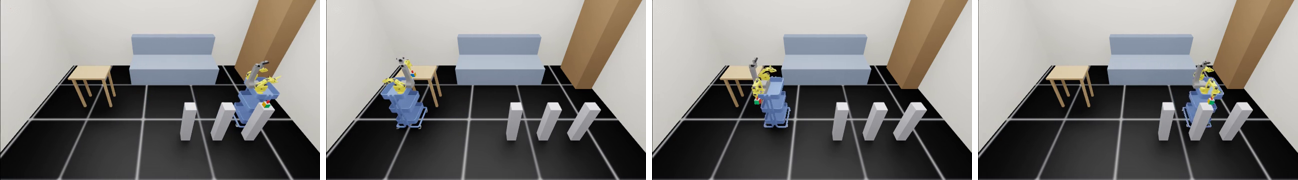
\includegraphics[width=\stripw]{putitback_overview.png}\\[2pt]
\rowlabel{Head camera} & 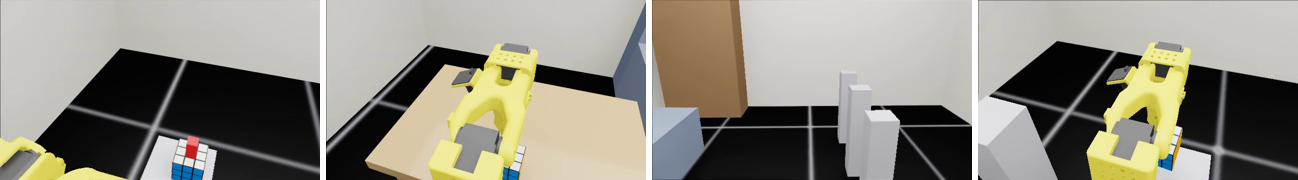
\includegraphics[width=\stripw]{putitback_head.png}\\[2pt]
\rowlabel{Wrist camera} & 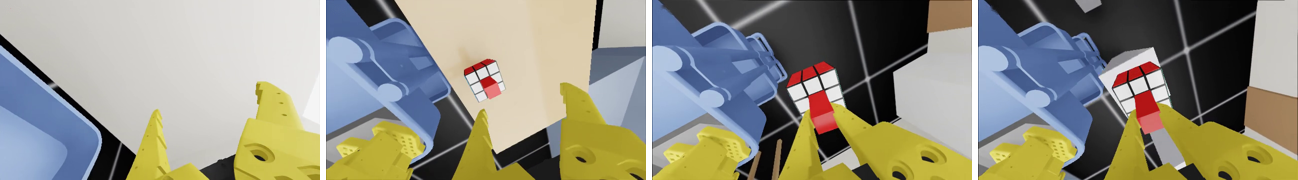
\includegraphics[width=\stripw]{putitback_wrist.png}\\
\end{tabular}
\caption{The see--detour--act pattern shared by all tasks, shown on PutItBack in simulation (one episode of the scripted expert). Rows: a third-person chase view, which the policy does not get, the head camera and the right wrist camera. (1)~The head camera sees the $2{\times}2{\times}4$\,cm block on one of three identical stations, and the robot picks it up. (2)~It drives the block to the work table; facing the table, no camera shows the stations. (3)~It turns back: the three stations look the same whatever the block's start was, so only memory says where to go. (4)~It puts the block back on the station it came from. The visible twin keeps the cue readable in the act phase and changes nothing else, so it removes only the need to remember.}
\label{fig:pattern}
\end{figure*}

\textbf{Memory in VLA policies.} RoboMME~\cite{dai2026robomme} studies past frames, language subgoals and recurrent states as memory for \pizf{}, fed into the model as extra context, as a modulator of the action expert, or as a separate memory expert. MemER~\cite{sridhar2026memer} trains a high-level policy to select keyframes and to instruct a low-level VLA. MEM~\cite{torne2026mem} combines short video context with language notes for tasks that last many minutes. SOMA~\cite{li2026soma} scans the workspace with a movable head camera and stores what it saw in a spatial memory. These are the memory families we compare, using RoboMME's ways of feeding memory into the model.

\textbf{Memory for mobile manipulation.} EchoVLA~\cite{lin2025echovla} adds a scene memory and an episodic memory to a VLA. MessyMem~\cite{banwasi2026messymem} builds a persistent memory from the robot's own interactions over hours of household tasks. DynaMem~\cite{liu2024dynamem} keeps a 3D memory that is updated as objects move, and ESCAPE~\cite{qian2026escape} couples an episodic spatial memory with a policy that switches between navigation and manipulation. All are methods, tested on long tasks of their own. Storing each observation with the pose it was taken from goes back to the Scene Memory Transformer~\cite{fang2019smt}, and ReMEmbR~\cite{anwar2024remembr} retrieves a robot's history by position as well as by time; we use this idea as one memory variant inside a VLA. DetourMem complements these methods with short, controlled tasks in which only the memory demand changes. To our knowledge no existing benchmark pairs each mobile memory task with a visible twin or treats the time and distance away as a controlled factor.

\textbf{Low-cost mobile manipulation.} Mobile ALOHA~\cite{fu2025mobilealoha} showed that a low-cost two-arm mobile robot can learn household tasks from about 50 demonstrations per task when co-trained with static-arm data. XLeRobot~\cite{wang2025xlerobot} lowers the cost further and is supported by the LeRobot software stack~\cite{cadene2026lerobot}, so the real-robot part of a benchmark does not need a rare robot.

\section{Problem Statement and Hypotheses}
\label{sec:problem}

\textbf{Setting.} We treat each task as a partially observable decision problem~\cite{kaelbling1998pomdp}. At step $t$ the policy receives an observation $o_t$ (one head-camera image, two wrist-camera images, joint positions and base velocity) and a language instruction $\ell$. A \emph{memoryless} policy has the form $\pi(a_t \mid o_t, \ell)$. A \emph{memory} policy has the form $\pi(a_t \mid o_t, m_t, \ell)$, where $m_t = f(o_{1:t-1})$ is whatever the method keeps from the past: frames, notes, a path or a map.

\textbf{Episode structure.} Each episode has a hidden cue $c$ drawn from a finite set $C$: which station, which bin, how many, which route. In the \emph{cue phase} the robot can see $c$. In the \emph{gap phase} it drives a detour of duration $\Delta$ and path length $d$, during which no camera shows $c$ or anything that gives it away. In the \emph{act phase} the right action depends on $c$ (Fig.~\ref{fig:pattern}).

\textbf{Memory dependence.} A task is memory-dependent if the observations at the start of the act phase have the same distribution for every cue in $C$. Under the scoring rule of R4 (Section~\ref{sec:rules}), a memoryless policy then cannot do better than chance, however well it drives and grasps.

\textbf{Measures.} Let $\Smem$ be the success rate on a task and $\Svis$ that of the same policy on its visible twin. Each task is also split into ordered subgoals, each tagged as a \emph{memory decision} (which table to drive to) or as \emph{execution} (a grasp or place whose target is known); PyramidTour has nine: three table choices, three grasps and three placements. The \emph{subgoal score} $\SG$ is the fraction of subgoals completed before the first failure, following the staged partial success of HomeRobot OVMM~\cite{yenamandra2023homerobot} and the chain length of CALVIN~\cite{mees2022calvin}. The chance level $\kappa$ of a measure is the value reached by the scripted expert (Section~\ref{sec:demos}) when it guesses at every memory decision; for a single choice among $|C|$ options this is $1/|C|$. We report the \emph{memory gap} $G = \Svis - \Smem$ and the \emph{memory score}
\begin{equation}
M = \frac{\Smem - \kappa}{\Svis - \kappa},
\label{eq:memscore}
\end{equation}
which is 0 for a policy that guesses and 1 for a policy that loses nothing when the cue is hidden, and compute both in the same way from $\SG$. $M$ is only reported when $\Svis$ is clearly above $\kappa$.

\textbf{Hypotheses.}

\textbf{H1} \emph{Memoryless VLAs fail, and for the expected reason.} After fine-tuning, \pizf{} and GR00T reach high $\Svis$ but stay near $\kappa$ on the memory tasks. Their failures are wrong choices (a clean grasp at the wrong station), not failed motions.

\textbf{H2} \emph{Memory helps, less so with longer absence, and each kind where it fits.} Adding memory lifts $M$ above 0. $M$ falls as $\Delta$ and $d$ grow, fastest for time-indexed frames, whose fixed budget has to cover a longer gap. Each memory does best on the suite whose cue it stores: pose-indexed frames and the object map on Return and Survey, event notes on Loop and on symbolic Transfer cues, the odometry trace and time-indexed frames on Path. On the capstone task no single memory is enough.

\textbf{H3} \emph{Leaving is harder than waiting.} For the same time out of view, $M$ is lower when the robot drives away and comes back than when it stays in place and a screen hides the cue, because the returning robot sees the scene from a slightly different pose. If so, looking memory up by place should narrow this gap more than looking it up by time.

\textbf{H4} \emph{Simulation predicts the real robot in ranking, not in level.} On the mirrored tasks, the order of the methods and the trend over absence are the same in simulation and on the real robot, although absolute success is lower on the real robot.

H3 is specific to mobile robots. If it is false, tabletop memory benchmarks already tell us what we need to know for mobile manipulation, which would be worth knowing because tabletop tests are cheaper.

\section{Benchmark Design}

\subsection{Design Rules}
\label{sec:rules}

\textbf{R1: The cue leaves view through the robot's own motion.} The base moves, or the head camera turns away as part of the task. Covers or screens are used only in the ``waiting'' condition of H3.

\textbf{R2: Same view, different history.} At the start of the act phase the scene must look the same for all cues, e.g.\ three identical stations with an empty slot each. We check this automatically (Section~\ref{sec:demos}).

\textbf{R3: A visible twin.} The twin uses the same scene, route and motions, with one change that keeps the cue readable in the act phase (a marker that stays on, an open container, a line on the floor) and is not easier in any other way. It is part of training and testing.

\textbf{R4: A known chance level.} The act phase is a choice among $K$ options, an order of $K$ options, or a count up to a known maximum. Because a mobile robot could simply drive over and look again, the option it first commits to (drives up to or opens) is the one that counts; reaching a wrong option first is a wrong choice.

\textbf{R5: The robot gathers the cue itself} with its own head camera while it moves through the scene, so that looking is part of the skill.

\subsection{Absence as a Controlled Factor}

Each task comes at three absence levels: the cue is out of view for roughly 10\,s, 30\,s and 90\,s, with detours of about 1\,m, 3\,m and 6\,m. To pull time and distance apart, two conditions are added on a subset of tasks: a long wait after a short drive, and the ``waiting'' condition of H3, in which the robot does not drive and a screen hides the cue. The waiting condition is run on PutItBack, CarryTheCode and WhereDidItGo.

\subsection{Tasks}
\label{sec:tasks}

Table~\ref{tab:tasks} lists the 14 tasks: 13 core tasks in five suites and one capstone task. Tabletop benchmarks group tasks by the type of memory~\cite{dai2026robomme}. On a mobile robot a second question matters as much: where the cue is seen compared with where the robot must act. We group the tasks by this relation into five suites, each targeting one kind of mobile memory: in \emph{Return} the cue is one of $K$ look-alike places that the robot leaves and must come back to; in \emph{Transfer} it is seen at one place and used at another; in \emph{Survey} it is spread over several places seen on a tour; in \emph{Path} it is the robot's own route or order of visits; and in \emph{Loop} it builds up over repeated trips. In every core task the remembered cue decides where the base goes, and in most it also decides what the arms do there. We use $K = 3$ by default. For SearchWithoutRepeats and DeliverToEach there is no single correct choice, so we report repeated visits and compare them with the guessing expert. TourThenFetch asks for one item and PyramidTour for three in a fixed order; CarryTheCode carries a symbol to another place, WhereDidItGo an identity tracked while the boxes move. The capstone task, ChillAndServe, combines progress, place and order in time. It is reported separately and tests whether a memory's per-suite profile predicts how it does when several demands meet.

\begin{table*}[t]
\centering
\caption{The 14 tasks of DetourMem, grouped by suite, with the kind of memory each suite targets. Tasks marked $*$ are mirrored on the real robot.}
\label{tab:tasks}
\footnotesize
\renewcommand{\arraystretch}{1.15}
\begin{tabularx}{\textwidth}{@{}l >{\raggedright\arraybackslash}X >{\raggedright\arraybackslash}p{4.3cm} c@{}}
\toprule
Task & What the robot does and what it must remember & What the visible twin changes & Chance \\
\midrule
\multicolumn{4}{@{}l}{\textbf{Return} (place memory)} \\
\addlinespace[2pt]
PutItBack$^*$ & Pick up a $2{\times}2{\times}4$\,cm block from one of $K$ identical 70\,cm stations, take it to a work table, turn back and return it to its station. \emph{Remember: the origin station.} & A marker stays on the origin station. & $1/K$ \\
StashAndRetrieve & A flag marks one of $K$ closed bins around the room; the robot puts a cube in it, the flags are removed, and after an errand it fetches the cube. \emph{Remember: which bin.} & The bins stay open. & $1/K$ \\
\addlinespace[5pt]
\multicolumn{4}{@{}l}{\textbf{Transfer} (carry-over memory)} \\
\addlinespace[2pt]
CarryTheCode$^*$ & A coloured card at station A names one of $K$ bins; the robot fetches a cube from shelf B and delivers it to that bin. \emph{Remember: the colour.} & A panel at the bins repeats the colour. & $1/K$ \\
MatchAndFetch & See a sample object at the work table, drive to $K$ storage stations and bring back the matching object. \emph{Remember: the sample.} & A picture of the sample hangs at the stations. & $1/K$ \\
WhereDidItGo & One of $K$ identical boxes is marked, then the boxes are carried to $K$ stations while the robot watches; after a detour it fetches the marked box. \emph{Remember: where that box went.} & The box carries a tag. & $1/K$ \\
\addlinespace[5pt]
\multicolumn{4}{@{}l}{\textbf{Survey} (map memory)} \\
\addlinespace[2pt]
TourThenFetch & Tour $K$ stations with different items, then bring a requested item from the station that had it. \emph{Remember: what is where.} & Stations carry labels readable from afar. & $1/K$ \\
PyramidTour$^*$ & Tour three tables, each holding one piece of a pyramid; from the assembly table, fetch and stack base, middle and top in order. \emph{Remember: which table holds which piece.} & Each table carries a sign naming its piece. & $1/K!$ \\
ResetTheRoom & Tour $K$ stations with different items; the items are gathered into one tray while the robot is away; put each back. \emph{Remember: the layout.} & Each station shows a picture of its item. & $1/K!$ \\
SearchWithoutRepeats & Search $K$ closed containers around the room for an object, with a detour in between, without opening one twice. \emph{Remember: what was checked.} & Checked containers stay open. & see text \\
\addlinespace[5pt]
\multicolumn{4}{@{}l}{\textbf{Path} (trajectory memory)} \\
\addlinespace[2pt]
RouteReplay & Be driven once along one of $K$ routes, return to the start, then repeat the route alone. \emph{Remember: the route.} & The route is taped on the floor. & $1/K$ \\
VisitInOrder & Be driven once to $K$ stations in some order, then deliver one item to each in that order. \emph{Remember: the order.} & Stations carry numbered signs. & $1/K!$ \\
\addlinespace[5pt]
\multicolumn{4}{@{}l}{\textbf{Loop} (progress memory)} \\
\addlinespace[2pt]
ShuttleXTimes$^*$ & Carry cubes one per trip to an opaque box across the room and stop once $N$ have been delivered. \emph{Remember: how many so far.} & Open tray; delivered cubes can be counted. & $1/4$ \\
DeliverToEach & Deliver one item per trip to each of $K$ identical stations, into opaque boxes, without serving a station twice. \emph{Remember: which were served.} & The boxes are open. & see text \\
\addlinespace[5pt]
\multicolumn{4}{@{}l}{\textbf{Capstone} (progress, place and order in time; reported separately)} \\
\addlinespace[2pt]
ChillAndServe & Put identical cans one per trip into fridge slots marked only while a can goes in; when told a can is ready, take out the oldest. \emph{Remember: the slots and their order.} & Each slot shows its insertion number. & $1/N$ \\
\bottomrule
\end{tabularx}
\end{table*}

\subsection{Robot and What It Allows}

XLeRobot~\cite{wang2025xlerobot} carries two arms with five joints and a gripper each on an omnidirectional base, with a pan-tilt head camera and one camera at each wrist. The action has 17 dimensions: 12 arm and gripper joint targets, 2 head joint targets and 3 base velocities. The arms reach about 0.4\,m and carry well under 1\,kg, and the body height is fixed. All surfaces are therefore at one reachable height, objects are light and grasped from above (cubes, cups, small boxes, pyramid pieces with a common grip tab), lids and doors are light flip or magnetic covers, and partitions keep the stations out of each other's view. Manipulation stays simple on purpose, so that the twins are solvable and what remains hard is the memory.

\section{Demonstration Generation}
\label{sec:demos}

Teleoperating a two-arm mobile robot through hundreds of episodes per task is slow, and human operators know the cue and can act on it in ways that leave no trace in the images. We therefore generate most demonstrations with scripted experts in simulation.

\textbf{Simulated twin.} We build the robot in Isaac Lab~\cite{mittal2023orbit}, starting from the models and data tools of LeIsaac~\cite{leisaac2025}, and record in the LeRobot format~\cite{cadene2026lerobot} with the same 17 action dimensions and three cameras as the real robot. Simulated joint angles and real motor readings are tied by a per-joint linear map fitted from a few reference poses.

\textbf{Experts that only use what was seen.} An expert with full access to the simulator would drive to the right station because it reads the answer from the simulator state, and such data would teach a policy to guess. For \emph{how} to move (grasp poses, arm paths, base waypoints) the expert may use the simulator state. For \emph{what} to do (which station, how many more, where to return) it may only read a belief store, which a fact enters only when the object or event was inside a camera frustum, not occluded, and covered enough pixels. Where the cue has to be looked for, the expert turns the head camera first. The same expert, with every memory decision replaced by a random choice, gives the chance level $\kappa$ of each measure.

\textbf{Checks.} A replay check confirms that the cue was visible in the cue phase and in no frame of the gap and act phases (R1, R2). A shortcut test trains a memoryless policy on each task alone; if it beats chance clearly, the task leaks the cue and we fix the scene.

\textbf{Variation and size.} Object poses, colours, distractors, lighting, the detour route and the absence level are sampled per episode, and instructions come from several templates. We plan 100 demonstrations per task and version (memory task or twin), and 50 held-out test episodes per task, version and absence level, with the same seeds for every method.

\textbf{Real robot.} For the mirrored tasks we add a small number of teleoperated demonstrations (Joy-Con controllers) and co-train on simulated and real data, following Mobile ALOHA~\cite{fu2025mobilealoha}. The operator follows the expert's subtask order, and demonstrations in which the robot moves towards an option before the cue was seen are discarded.

\section{Evaluation Plan}

\textbf{Policies.} All memory variants use the \pizf{} backbone and RoboMME's ways of feeding memory into it~\cite{dai2026robomme}: image memories modulate the action expert, text memories are added to the context. Every variant gets the same budget of memory tokens per step, the same data and the same number of training steps.
\begin{itemize}
\item \emph{No memory.} \pizf{}~\cite{black2025pi05} and GR00T~\cite{bjorck2025gr00t}, so that H1 does not rest on one model.
\item \emph{V1: Time-indexed frames.} Past head-camera frames sampled over the episode, added through feature modulation, RoboMME's best way of adding frames. This is the tabletop baseline.
\item \emph{V2: Pose-indexed frames.} The same frames and budget, each tagged with the head camera's pose from the integrated base velocities and head joints. The frames taken closest to the current pose, or to the place the instruction refers to, are selected and their relative pose is added as an embedding~\cite{fang2019smt,anwar2024remembr}. V1 and V2 differ only in whether memory is looked up by \emph{when} or by \emph{where} it was seen.
\item \emph{V3: Odometry trace.} No images: the robot's base path, relative to its current pose, with markers where the gripper closed or opened, written into the context.
\item \emph{V4: Event notes.} A small vision-language model keeps a few keyframes and writes a short note at events (``two cubes delivered'', ``the card was red'') for the low-level policy, in the spirit of MemER~\cite{sridhar2026memer} and MEM~\cite{torne2026mem}.
\item \emph{V5: Object map.} Objects seen by the head camera are placed in a map using odometry, and the entries matching the instruction are given relative to the robot, in the spirit of SOMA~\cite{li2026soma} and EchoVLA~\cite{lin2025echovla}.
\item \emph{Oracle memory.} The true cue is written into the instruction. This is not a method; it shows how well the policy could do with perfect memory.
\end{itemize}
On the capstone task we also run V4 and V5 together. One multi-task policy is trained per method on all tasks and twins, so that the only difference between $\Smem$ and $\Svis$ is whether the cue can be seen. V2, V3 and V5 rely on odometry, so we run them in simulation with exact pose and with odometry noise matched to the real robot.

\textbf{What we measure.} (i)~$S$ and $\SG$ per task, twin and absence level, with 95\% intervals (Wilson for $S$, bootstrap for $\SG$). (ii)~$G$ and $M$ for both. (iii)~Decision accuracy, the share of memory decisions at which the first commitment is right, and an error split of each failure into a \emph{wrong choice} or an \emph{execution failure}; H1 predicts the first kind dominates. (iv)~$M$ over absence, for driving away and for waiting (H2, H3); their difference at equal time away is the main mobile-specific number. (v)~The rank agreement of methods between simulation and the real robot (H4). (vi)~Inference time and tokens per step. On the real robot, subgoals and choices are annotated from video.

\textbf{Real robot.} Four tasks are mirrored, one per suite except Path, where odometry drift would mix with the memory effect: PutItBack, CarryTheCode, PyramidTour and ShuttleXTimes, each with its twin at two absence levels and 20 trials per condition.

\textbf{Pilot.} The same four tasks and twins come first in simulation, with the memoryless policies and oracle memory. This is the smallest experiment that can confirm or reject H1 and that shows whether the twins are solvable and the tasks do not leak. The first memory comparison is then V1 against V2.

\section{Expected Insights, Including From Negative Results}
\label{sec:insights}

\emph{Memoryless policies beat chance on a memory task.} The task leaks the cue; we report what the policy used (a shadow, a pose difference, the timing of the detour) and repair it. A benchmark whose shortcuts have been found is worth more than one where nobody looked.

\emph{Memoryless policies fail on the twins as well.} The tasks are too hard for the robot or the data; we simplify manipulation until the twins are solved.

\emph{Memory variants do not beat no memory, while the oracle does.} The information is there but the policy does not learn to use it, which points at training, not architecture. \emph{If the oracle is also poor}, the act phase itself is the bottleneck and the task measures the wrong thing.

\emph{$M$ does not fall with absence.} Time and distance are not what makes remembering hard at this scale; we would vary the number of distractors and of things to remember instead.

\emph{Waiting is as hard as leaving (H3 rejected).} Tabletop memory benchmarks carry over to mobile robots, and the cheaper tests can be used with more confidence. \emph{Pose-indexed frames do no better than time-indexed ones.} At the distances a small robot covers, the frame memory used on tabletops is enough.

\emph{No single memory wins.} We expect this from the tabletop results~\cite{dai2026robomme} and from H2. A per-suite table of which memory helps where would be the main practical result. \emph{If per-suite results do not predict the capstone task}, memories do not simply add up when several demands meet.

\emph{Simulation and real robot disagree in ranking.} We report on which tasks, and whether the cause is on the seeing side (camera, lighting) or the moving side (base slip, arm play).

\section{Limitations}

The benchmark uses one small robot whose reach, payload and fixed height rule out many household tasks, so results may not carry over to larger platforms. Scripted demonstrations are cleaner than human ones, which may make the twins easier than real use. Absences last minutes and metres, not the hours and rooms that persistent-memory systems aim at~\cite{banwasi2026messymem}. Base odometry drifts, which may hurt the pose-based memories (V2, V3, V5) on the real robot; the simulated odometry noise is meant to show this in advance. WhereDidItGo, ResetTheRoom, SearchWithoutRepeats and the capstone task need a person to move objects or light containers and doors, so they are run in simulation first.

%% Use plainnat to work nicely with natbib.
\renewcommand{\bibfont}{\footnotesize}
\setlength{\bibsep}{1pt}
\bibliographystyle{plainnat}
\bibliography{references}

\end{document}